\subchapter{Lab1: First Yocto Project build}{Your first dive into Yocto
Project and its build mechanism}

During this lab, you will:
\begin{itemize}
  \item Set up an OpenEmbedded environment
  \item Configure the project and choose a target
  \item Build your first Poky image
\end{itemize}

\section{Setup}

Before starting this lab, make sure your home directory is not
encrypted using eCryptFS. OpenEmbedded cannot be used on top of an eCryptFS file
system due to limitations in file name lengths.

Go to the \code{$HOME/__SESSION_NAME__-labs/} directory.

Install the required packages:
\begin{bashinput}
sudo apt install bc build-essential chrpath cpio diffstat gawk git python3 texinfo wget lz4
\end{bashinput}

\section{Download Yocto}

Download the \code{kirkstone} version of Poky:
\begin{bashinput}
git clone https://git.yoctoproject.org/git/poky
cd $HOME/__SESSION_NAME__-labs/poky
git checkout -b kirkstone-4.0.17 kirkstone-4.0.17
\end{bashinput}

Return to your project root directory (\code{cd $HOME/__SESSION_NAME__-labs/})
and download the \code{meta-openembedded}, \code{meta-arm} and \code{meta-ti} layers:
\begin{bashinput}
cd $HOME/__SESSION_NAME__-labs
git clone -b kirkstone https://git.openembedded.org/meta-openembedded
git clone https://git.yoctoproject.org/git/meta-arm
cd meta-arm
git checkout -b yocto-4.0.3 yocto-4.0.3
\end{bashinput}
\begin{bashinput}
cd $HOME/__SESSION_NAME__-labs
git clone https://git.yoctoproject.org/git/meta-ti
cd meta-ti
git checkout -b kirkstone-labs 1899f5ead39d88e18442209f06d23a8c291f978a
git am $HOME/__SESSION_NAME__-labs/bootlin-lab-data/0001-Use-extlinux.conf-booting-flow.patch
\end{bashinput}

\section{Set up the build environment}

Check you're using Bash. This is the default shell when using Ubuntu.

Export all needed variables and set up the build directory:
\begin{bashinput}
cd $HOME/__SESSION_NAME__-labs
source poky/oe-init-build-env
\end{bashinput}

You must specify which machine is your target. By default it
is \code{qemu}. We need to build an image for a \code{beagleplay}.
Update the \yoctovar{MACHINE} configuration variable accordingly. Be
careful, \code{beagleplay} is different from the \code{beagleboard}
or the \code{beaglebone} machines!

Also, if you need to save disk space on your computer you can add \code{INHERIT
+= "rm_work"} in the previous configuration file. This will remove the
package work directory once a package is built.

Don't forget to make the configuration aware of the meta-openembedded, ARM and TI layers. Edit the
layer configuration file (\code{$BUILDDIR/conf/bblayers.conf}) and append the
full path to the \code{meta-oe}, \code{meta-arm-toolchain}, \code{meta-arm},
\code{meta-ti-bsp} directories to the \code{BBLAYERS} variable.

\section{Build your first image}

Now that you're ready to start the compilation, simply run:
\begin{bashinput}
bitbake core-image-minimal
\end{bashinput}

Once the build finished, you will find the output images under
\code{$BUILDDIR/tmp/deploy/images/beagleplay}.

\section{Set up the SD card}

In this first lab we will use an SD card to store the bootloader, kernel and
root filesystem files. The SD card image has been generated and is
named \code{core-image-minimal-beagleplay.wic.xz}.

Now uncompress and flash the image with the following command:
\begin{bashinput}
xz -dc $BUILDDIR/tmp/deploy/images/beagleplay/core-image-minimal-beagleplay.wic.xz | sudo dd of=/dev/sdX conv=fdatasync bs=4M status=progress
\end{bashinput}

\section{Setting up serial communication with the board}

The Beagle Play serial connector is a 3-pin header located right next to the
board's USB-C port. Using your special USB to Serial adapter provided  by your
instructor, connect the ground wire (blue) to the pin labeled "G", the
\code{TX} wire (red) to the pin labeled "RX" and the \code{RX} wire (green) to
the pin labeled "TX" \footnote{See \url{https://www.olimex.com/Products/Components/Cables/USB-Serial-Cable/USB-SERIAL-F/}
for details about the USB to Serial adapter that we are using.}.

You always should make sure that you connect the \code{TX} pin of the cable
to the \code{RX} pin of the board, and vice versa, whichever board and
cables you use.

\begin{center}
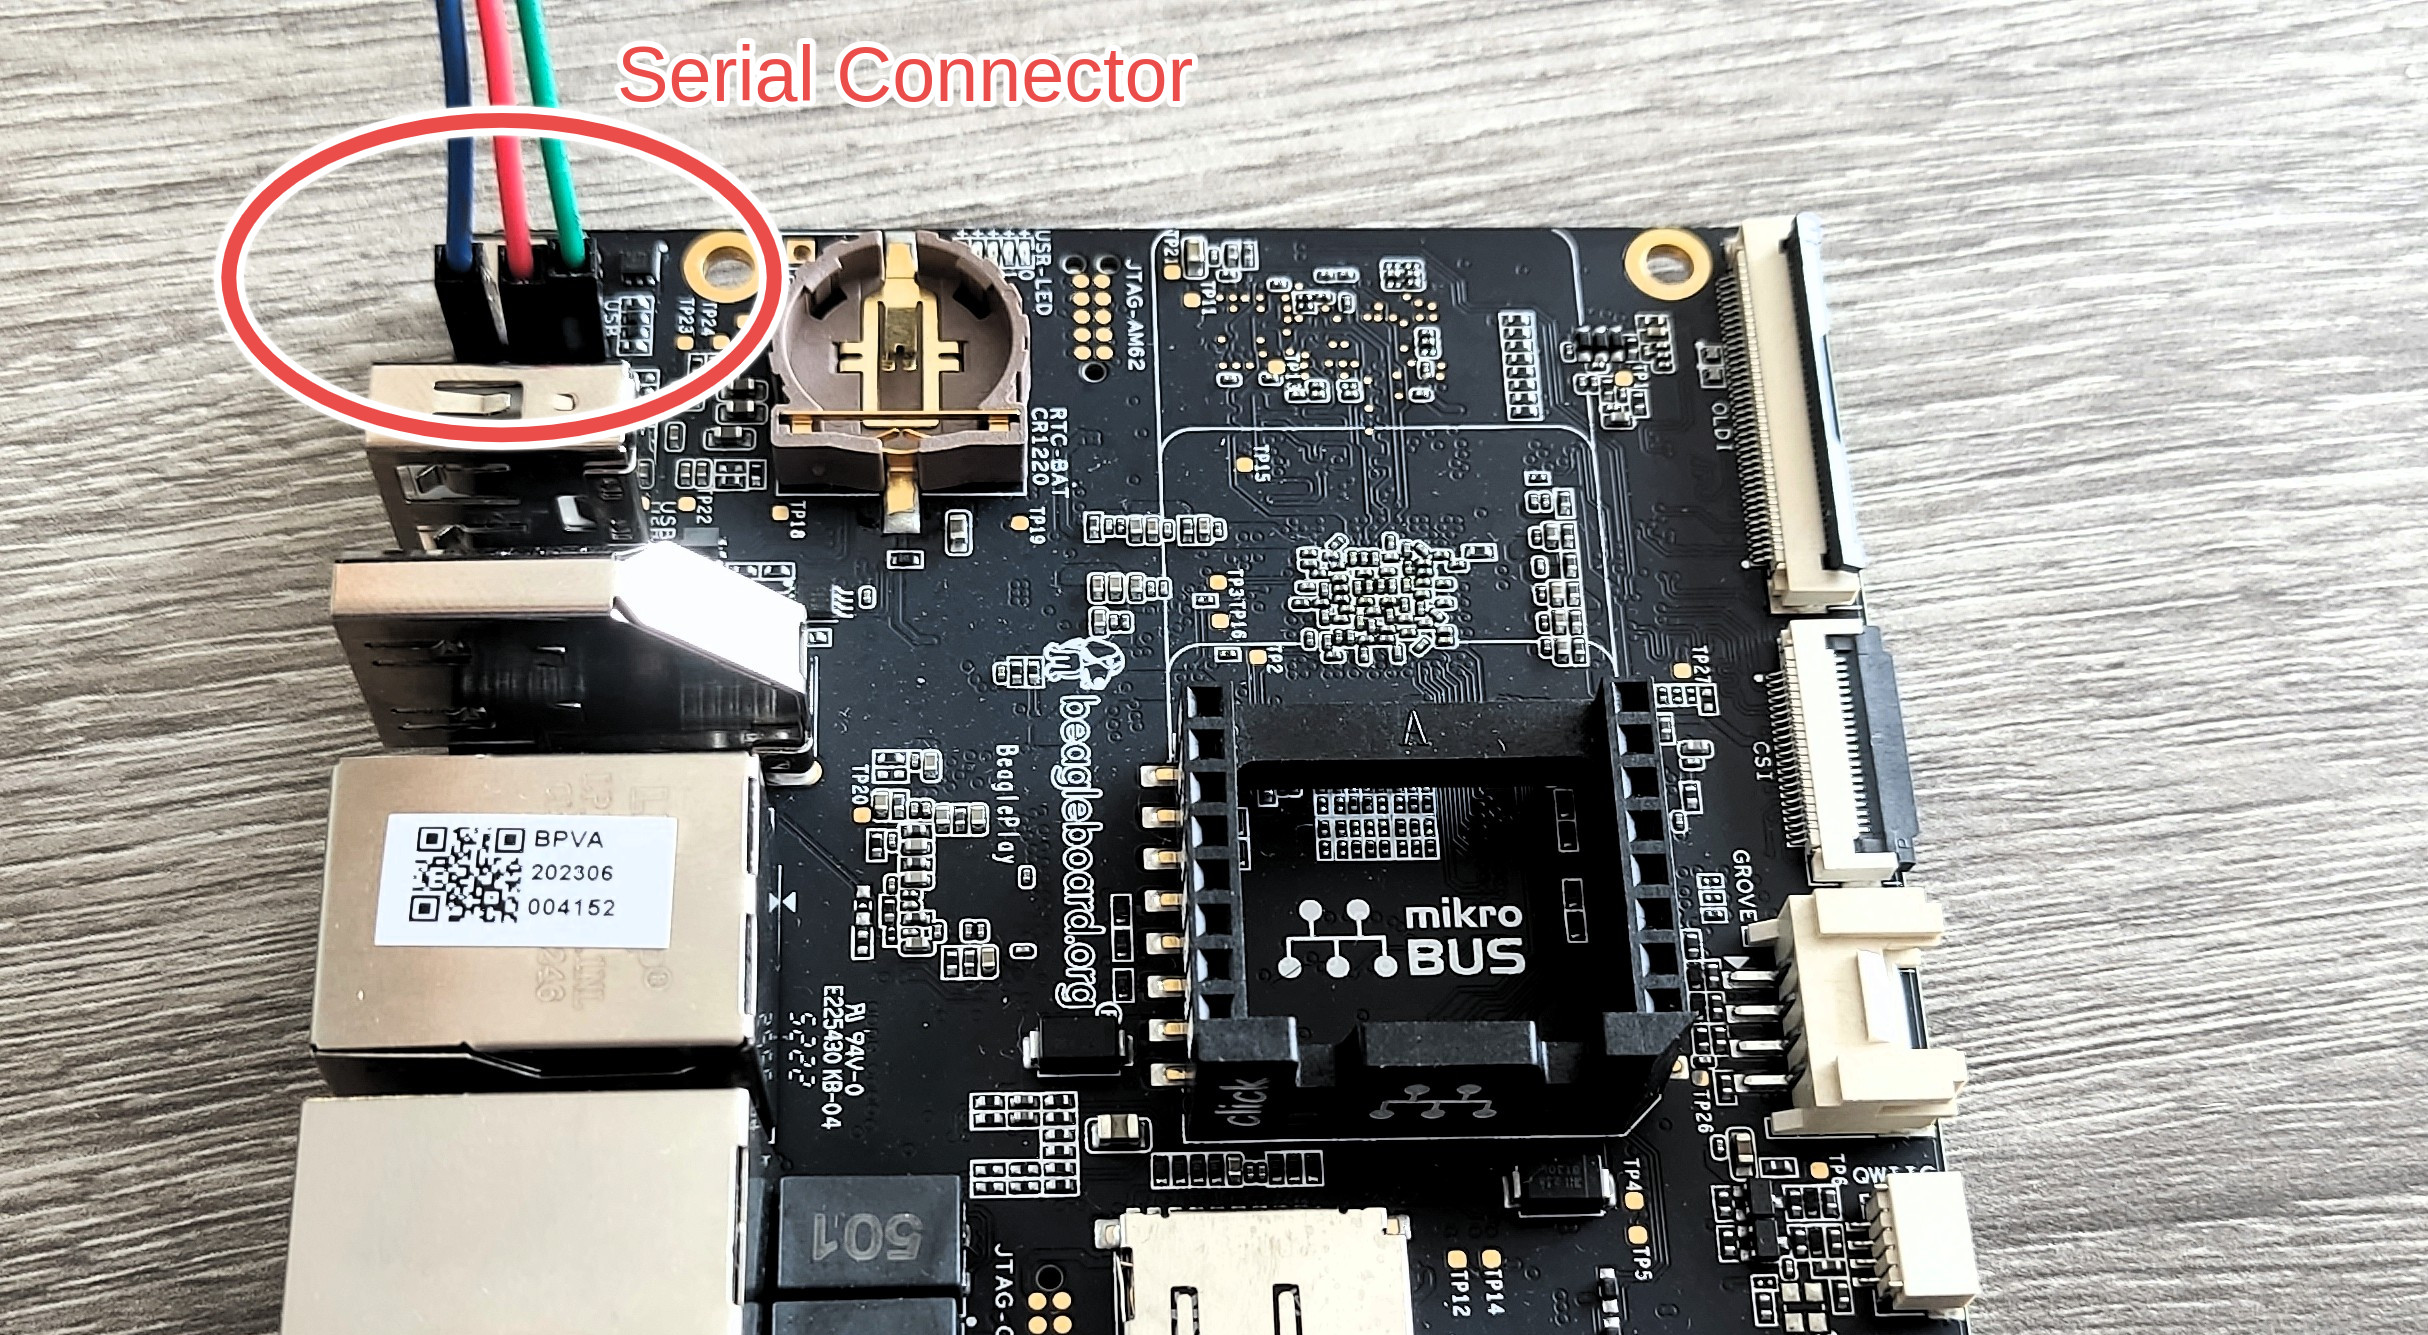
\includegraphics[width=8cm]{common/beagleplay-serial-connection.jpg}
\end{center}

Once the USB to Serial connector is plugged in, a new serial port
should appear: \code{/dev/ttyUSB0}.  You can also see this device
appear by looking at the output of \code{dmesg}.

To communicate with the board through the serial port, install a
serial communication program, such as \code{picocom}:

\begin{bashinput}
sudo apt install picocom
\end{bashinput}

If you run \code{ls -l /dev/ttyUSB0}, you can also see that only
\code{root} and users belonging to the \code{dialout} group have
read and write access to this file. Therefore, you need to add your user
to the \code{dialout} group:

\begin{bashinput}
sudo adduser $USER dialout
\end{bashinput}

{\bf Important}: for the group change to be effective, in Ubuntu 18.04, you have to
{\em completely reboot} the system \footnote{As explained on
\url{https://askubuntu.com/questions/1045993/after-adding-a-group-logoutlogin-is-not-enough-in-18-04/}.}.
A workaround is to run \code{newgrp dialout}, but it is not global.
You have to run it in each terminal.

Now, you can run \code{picocom -b 115200 /dev/ttyUSB0}, to start serial
communication on \code{/dev/ttyUSB0}, with a baudrate of \code{115200}. If
you wish to exit \code{picocom}, press \code{[Ctrl][a]} followed by
\code{[Ctrl][x]}.

There should be nothing on the serial line so far, as the board is not
powered up yet.

\section{Boot}

Insert the SD card in the dedicated slot on the BeaglePlay. Press the USR
push button, plug in the USB-C cable and
release the push button. You should see U-Boot messages on the console.
Stop the autoboot process by typing SPACE BAR and run the following commands:

\begin{verbatim}
  setenv boot_targets mmc1
  boot
\end{verbatim}

You should see Linux boot messages on the console.
Wait until the login prompt, then enter \code{root} as user.
Congratulations! The board has booted and you now have a shell.
